\documentclass[11pt]{article}
\usepackage[margin=1in]{geometry}
\usepackage{amsmath}
\usepackage{amssymb}
\usepackage{tikz}
\usepackage{pgfplots}
\pgfplotsset{compat=1.18}
\usepackage{graphicx}
\usepackage{fancyhdr}
\usepackage{enumitem}

\pagestyle{fancy}
\fancyhf{}
\rhead{AP PreCalculus FRQ 3 Practice}
\lhead{Modeling a Periodic Context}
\cfoot{\thepage}

\title{\textbf{AP PreCalculus}\\FRQ 3 Practice Questions\\Modeling a Periodic Context}
\author{15 Minutes - No Calculator}
\date{}

\begin{document}

\maketitle

\section*{Contents}
\begin{itemize}[noitemsep]
    \item Question 1: Ferris Wheel
    \item Question 2: Ocean Tide
    \item Question 3: Pendulum Swing
    \item Question 4: Trampoline Bounce
    \item Question 5: Temperature Variation
\end{itemize}

\newpage

\section*{Question 1: Ferris Wheel}

The Sky View Ferris wheel at the county fair takes passengers on a smooth, circular ride. At time $t = 0$ seconds, passenger Emma's seat is at the lowest point of the ride, 6 feet above the ground, modeled by $h(0) = 6$. As the wheel turns, Emma's seat reaches a maximum height of 86 feet above the ground. The Ferris wheel completes 20 full rotations in 60 seconds. The sinusoidal function $h$ models the height of Emma's seat above the ground, in feet, as a function of time $t$ in seconds, $0 \leq t \leq 60$.

\subsection*{(A)}
The graph of $h$ and its dashed midline for two full cycles is shown. Five points, $F$, $G$, $J$, $K$, and $P$, are labeled on the graph. No scale is indicated, and no axes are presented.

Determine possible coordinates $(t, h(t))$ for the five points: $F$, $G$, $J$, $K$, and $P$.

\begin{center}
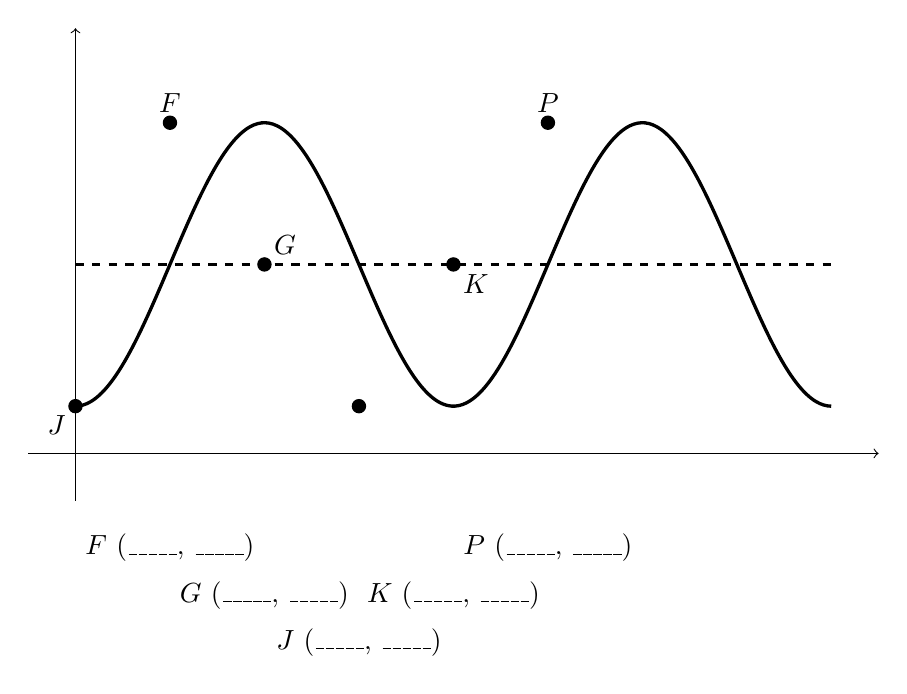
\begin{tikzpicture}[scale=1.2]
    % Draw axes (light)
    \draw[->] (-0.5,0) -- (8.5,0);
    \draw[->] (0,-0.5) -- (0,4.5);
    
    % Draw midline (dashed)
    \draw[dashed, thick] (0,2) -- (8,2);
    
    % Draw sinusoidal curve (starting at minimum)
    \draw[very thick, domain=0:8, samples=200, smooth] 
        plot (\x, {2 - 1.5*cos(90*\x)});
    
    % Mark and label points
    \filldraw (0,0.5) circle (2pt) node[below left] {$J$};
    \filldraw (1,3.5) circle (2pt) node[above] {$F$};
    \filldraw (2,2) circle (2pt) node[above right] {$G$};
    \filldraw (3,0.5) circle (2pt);
    \filldraw (4,2) circle (2pt) node[below right] {$K$};
    \filldraw (5,3.5) circle (2pt) node[above] {$P$};
    
    % Coordinate blanks
    \node at (1,-1) {$F$ (\_\_\_\_\_, \_\_\_\_\_)};
    \node at (5,-1) {$P$ (\_\_\_\_\_, \_\_\_\_\_)};
    \node at (2,-1.5) {$G$ (\_\_\_\_\_, \_\_\_\_\_)};
    \node at (4,-1.5) {$K$ (\_\_\_\_\_, \_\_\_\_\_)};
    \node at (3,-2) {$J$ (\_\_\_\_\_, \_\_\_\_\_)};
\end{tikzpicture}
\end{center}

\subsection*{(B)}
The function $h$ can be written in the form $h(t) = a \cos(b(t + c)) + d$. Find values of constants $a$, $b$, $c$, and $d$.

\begin{center}
\begin{tabular}{|l|}
\hline
$a = $ \underline{\hspace{3cm}} \\[10pt]
\hline
$b = $ \underline{\hspace{3cm}} \\[10pt]
\hline
$c = $ \underline{\hspace{3cm}} \\[10pt]
\hline
$d = $ \underline{\hspace{3cm}} \\[10pt]
\hline
\end{tabular}
\end{center}

\subsection*{(C)}
Refer to the graph of $h$ in part (A). The $t$-coordinate of $F$ is $t_1$, and the $t$-coordinate of $G$ is $t_2$.

\textbf{(i)} On the interval $(t_1, t_2)$, which of the following is true about $h$?

\begin{enumerate}[label=\alph*., leftmargin=1.5cm]
    \item $h$ is positive and increasing.
    \item $h$ is positive and decreasing.
    \item $h$ is negative and increasing.
    \item $h$ is negative and decreasing.
\end{enumerate}

\vspace{0.5cm}
\textbf{(ii)} Describe how the rate of change of $h$ is changing on the interval $(t_1, t_2)$.

\newpage

\section*{Question 1: SOLUTION}

\subsection*{(A) Coordinates}

\textbf{Work:}
\begin{itemize}[noitemsep]
    \item 20 rotations in 60 seconds = 1 rotation every 3 seconds
    \item Period = 3 seconds
    \item Max = 86 feet, Min = 6 feet
    \item Amplitude = $(86 - 6)/2 = 40$ feet
    \item Midline = $(86 + 6)/2 = 46$ feet
    \item Starting at minimum (cosine function at minimum)
    \item Increments of $3/4$ seconds between key points
\end{itemize}

\begin{center}
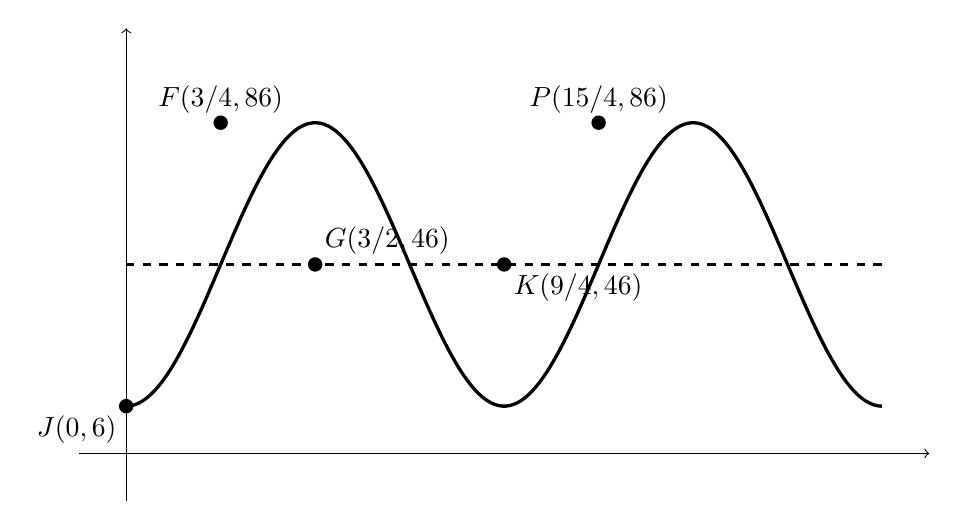
\begin{tikzpicture}[scale=1.2]
    % Draw axes (light)
    \draw[->] (-0.5,0) -- (8.5,0);
    \draw[->] (0,-0.5) -- (0,4.5);
    
    % Draw midline (dashed)
    \draw[dashed, thick] (0,2) -- (8,2);
    
    % Draw sinusoidal curve
    \draw[very thick, domain=0:8, samples=200, smooth] 
        plot (\x, {2 - 1.5*cos(90*\x)});
    
    % Mark and label points with coordinates
    \filldraw (0,0.5) circle (2pt) node[below left] {$J(0, 6)$};
    \filldraw (1,3.5) circle (2pt) node[above] {$F(3/4, 86)$};
    \filldraw (2,2) circle (2pt) node[above right] {$G(3/2, 46)$};
    \filldraw (4,2) circle (2pt) node[below right] {$K(9/4, 46)$};
    \filldraw (5,3.5) circle (2pt) node[above] {$P(15/4, 86)$};
\end{tikzpicture}
\end{center}

\begin{center}
\begin{tabular}{|c|c|}
\hline
$F(3/4, 86)$ & $P(15/4, 86)$ \\
\hline
$G(3/2, 46)$ & $K(9/4, 46)$ \\
\hline
\multicolumn{2}{|c|}{$J(0, 6)$} \\
\hline
\end{tabular}
\end{center}

\subsection*{(B) Constants}

\textbf{Work:}
\begin{itemize}[noitemsep]
    \item Amplitude: Since we start at minimum, $a = -40$
    \item Period = 3, so $\displaystyle\frac{2\pi}{b} = 3$, therefore $\displaystyle b = \frac{2\pi}{3}$
    \item Midline $d = 46$
    \item For cosine starting at minimum: $c = 0$
\end{itemize}

\begin{center}
\begin{tabular}{|l|}
\hline
$a = -40$ \\[10pt]
\hline
$b = 2\pi/3$ \\[10pt]
\hline
$c = 0$ \\[10pt]
\hline
$d = 46$ \\[10pt]
\hline
\end{tabular}
\end{center}

\textbf{Function:} $\displaystyle h(t) = -40 \cos\left(\frac{2\pi}{3} t\right) + 46$

\subsection*{(C) Function Behavior}

\textbf{(i) Answer: b. $h$ is positive and decreasing.}

On the interval $F$ to $G$ $(3/4$ to $3/2)$, the function decreases from the maximum (86 feet) to the midline (46 feet). Throughout this interval, $h$ remains positive.

\vspace{0.5cm}
\textbf{(ii) Rate of change description:}

Since $h$ is concave down on the entire interval $(3/4, 3/2)$, the rate of change of $h$ is decreasing throughout. The rate starts at zero at the maximum $(t = 3/4)$, becomes increasingly negative, and reaches its most negative value as it approaches the midline at $t = 3/2$.

\newpage

\section*{Question 2: Ocean Tide}

A marine biologist is studying the tidal water level at a coastal dock. At time $t = 0$ hours (midnight), the water level is at its midline height of 8 feet above the ocean floor, modeled by $h(0) = 8$. As the tide changes, the water level reaches a maximum height of 14 feet above the ocean floor. The dock experiences 2 complete tidal cycles every 24 hours. The sinusoidal function $h$ models the height of the water level above the ocean floor, in feet, as a function of time $t$ in hours, $0 \leq t \leq 24$.

\subsection*{(A)}
The graph of $h$ and its dashed midline for two full cycles is shown. Five points, $F$, $G$, $J$, $K$, and $P$, are labeled on the graph. No scale is indicated, and no axes are presented.

Determine possible coordinates $(t, h(t))$ for the five points: $F$, $G$, $J$, $K$, and $P$.

\begin{center}
\begin{tikzpicture}[scale=1.2]
    % Draw axes (light)
    \draw[->] (-0.5,0) -- (8.5,0);
    \draw[->] (0,-0.5) -- (0,4.5);
    
    % Draw midline (dashed)
    \draw[dashed, thick] (0,2) -- (8,2);
    
    % Draw sinusoidal curve (starting at midline, increasing)
    \draw[very thick, domain=0:8, samples=200, smooth] 
        plot (\x, {2 + 1.5*sin(90*\x)});
    
    % Mark and label points
    \filldraw (1,3.5) circle (2pt) node[above] {$F$};
    \filldraw (2,2) circle (2pt) node[above right] {$G$};
    \filldraw (3,0.5) circle (2pt) node[below] {$J$};
    \filldraw (4,2) circle (2pt) node[below right] {$K$};
    \filldraw (5,3.5) circle (2pt) node[above] {$P$};
    
    % Coordinate blanks
    \node at (1,-1) {$F$ (\_\_\_\_\_, \_\_\_\_\_)};
    \node at (5,-1) {$P$ (\_\_\_\_\_, \_\_\_\_\_)};
    \node at (2,-1.5) {$G$ (\_\_\_\_\_, \_\_\_\_\_)};
    \node at (4,-1.5) {$K$ (\_\_\_\_\_, \_\_\_\_\_)};
    \node at (3,-2) {$J$ (\_\_\_\_\_, \_\_\_\_\_)};
\end{tikzpicture}
\end{center}

\subsection*{(B)}
The function $h$ can be written in the form $h(t) = a \sin(b(t + c)) + d$. Find values of constants $a$, $b$, $c$, and $d$.

\begin{center}
\begin{tabular}{|l|}
\hline
$a = $ \underline{\hspace{3cm}} \\[10pt]
\hline
$b = $ \underline{\hspace{3cm}} \\[10pt]
\hline
$c = $ \underline{\hspace{3cm}} \\[10pt]
\hline
$d = $ \underline{\hspace{3cm}} \\[10pt]
\hline
\end{tabular}
\end{center}

\subsection*{(C)}
Refer to the graph of $h$ in part (A). The $t$-coordinate of $F$ is $t_1$, and the $t$-coordinate of $J$ is $t_2$.

\textbf{(i)} On the interval $(t_1, t_2)$, which of the following is true about $h$?

\begin{enumerate}[label=\alph*., leftmargin=1.5cm]
    \item $h$ is positive and increasing.
    \item $h$ is positive and decreasing.
    \item $h$ is negative and increasing.
    \item $h$ is negative and decreasing.
\end{enumerate}

\vspace{0.5cm}
\textbf{(ii)} Describe how the rate of change of $h$ is changing on the interval $(t_1, t_2)$.

\newpage

\section*{Question 2: SOLUTION}

\subsection*{(A) Coordinates}

\textbf{Work:}
\begin{itemize}[noitemsep]
    \item 2 cycles in 24 hours = 1 cycle every 12 hours
    \item Period = 12 hours
    \item Max = 14 feet, Min = 2 feet (by symmetry)
    \item Amplitude = $(14 - 2)/2 = 6$ feet
    \item Midline = 8 feet (given)
    \item At $t = 0$, $h(0) = 8$ (at midline, increasing)
    \item Increments of $12/4 = 3$ hours between key points
\end{itemize}

\begin{center}
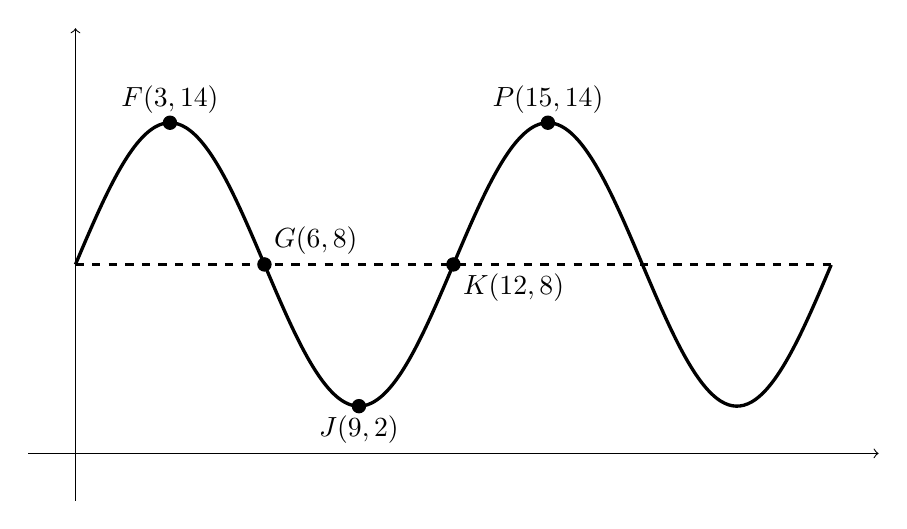
\begin{tikzpicture}[scale=1.2]
    % Draw axes (light)
    \draw[->] (-0.5,0) -- (8.5,0);
    \draw[->] (0,-0.5) -- (0,4.5);
    
    % Draw midline (dashed)
    \draw[dashed, thick] (0,2) -- (8,2);
    
    % Draw sinusoidal curve
    \draw[very thick, domain=0:8, samples=200, smooth] 
        plot (\x, {2 + 1.5*sin(90*\x)});
    
    % Mark and label points with coordinates
    \filldraw (1,3.5) circle (2pt) node[above] {$F(3, 14)$};
    \filldraw (2,2) circle (2pt) node[above right] {$G(6, 8)$};
    \filldraw (3,0.5) circle (2pt) node[below] {$J(9, 2)$};
    \filldraw (4,2) circle (2pt) node[below right] {$K(12, 8)$};
    \filldraw (5,3.5) circle (2pt) node[above] {$P(15, 14)$};
\end{tikzpicture}
\end{center}

\begin{center}
\begin{tabular}{|c|c|}
\hline
$F(3, 14)$ & $P(15, 14)$ \\
\hline
$G(6, 8)$ & $K(12, 8)$ \\
\hline
\multicolumn{2}{|c|}{$J(9, 2)$} \\
\hline
\end{tabular}
\end{center}

\subsection*{(B) Constants}

\textbf{Work:}
\begin{itemize}[noitemsep]
    \item Amplitude $a = 6$
    \item Period = 12, so $\displaystyle\frac{2\pi}{b} = 12$, therefore $\displaystyle b = \frac{\pi}{6}$
    \item Midline $d = 8$
    \item For sine starting at midline increasing: $c = 0$
\end{itemize}

\begin{center}
\begin{tabular}{|l|}
\hline
$a = 6$ \\[10pt]
\hline
$b = \pi/6$ \\[10pt]
\hline
$c = 0$ \\[10pt]
\hline
$d = 8$ \\[10pt]
\hline
\end{tabular}
\end{center}

\textbf{Function:} $\displaystyle h(t) = 6 \sin\left(\frac{\pi}{6} t\right) + 8$

\subsection*{(C) Function Behavior}

\textbf{(i) Answer: b. $h$ is positive and decreasing.}

On the interval $F$ to $J$ (3 to 9), the function decreases from the maximum (14 feet) to the minimum (2 feet). Throughout this interval, $h$ remains positive.

\vspace{0.5cm}
\textbf{(ii) Rate of change description:}

Since $h$ is concave down on the interval $(3, 6)$ and concave up on the interval $(6, 9)$, the rate of change of $h$ is negative throughout. On $(3, 6)$, the graph is concave down, so the rate of change is decreasing (becoming more negative). On $(6, 9)$, the graph is concave up, so the rate of change is increasing (becoming less negative, approaching zero).

\newpage

\section*{Question 3: Pendulum Swing}

A physics class is studying simple harmonic motion using a pendulum. At time $t = 0$ seconds, the pendulum bob is released from its maximum displacement of 18 inches to the right of center, modeled by $h(0) = 18$. As the pendulum swings, it passes through the center position and reaches a maximum displacement of 18 inches to the left of center. The pendulum completes 30 full swings in 45 seconds. The sinusoidal function $h$ models the horizontal distance of the pendulum bob from the center position, in inches, as a function of time $t$ in seconds, $0 \leq t \leq 45$. Positive values indicate displacement to the right, and negative values indicate displacement to the left.

\subsection*{(A)}
The graph of $h$ and its dashed midline for two full cycles is shown. Five points, $F$, $G$, $J$, $K$, and $P$, are labeled on the graph. No scale is indicated, and no axes are presented.

Determine possible coordinates $(t, h(t))$ for the five points: $F$, $G$, $J$, $K$, and $P$.

\begin{center}
\begin{tikzpicture}[scale=1.2]
    % Draw axes (light)
    \draw[->] (-0.5,0) -- (8.5,0);
    \draw[->] (0,-0.5) -- (0,4.5);
    
    % Draw midline (dashed)
    \draw[dashed, thick] (0,2) -- (8,2);
    
    % Draw sinusoidal curve (starting at maximum)
    \draw[very thick, domain=0:8, samples=200, smooth] 
        plot (\x, {2 + 1.5*cos(90*\x)});
    
    % Mark and label points
    \filldraw (0,3.5) circle (2pt) node[above left] {$F$};
    \filldraw (1,2) circle (2pt) node[above right] {$G$};
    \filldraw (2,0.5) circle (2pt) node[below] {$J$};
    \filldraw (3,2) circle (2pt) node[below right] {$K$};
    \filldraw (4,3.5) circle (2pt) node[above] {$P$};
    
    % Coordinate blanks
    \node at (1,-1) {$F$ (\_\_\_\_\_, \_\_\_\_\_)};
    \node at (5,-1) {$P$ (\_\_\_\_\_, \_\_\_\_\_)};
    \node at (2,-1.5) {$G$ (\_\_\_\_\_, \_\_\_\_\_)};
    \node at (4,-1.5) {$K$ (\_\_\_\_\_, \_\_\_\_\_)};
    \node at (3,-2) {$J$ (\_\_\_\_\_, \_\_\_\_\_)};
\end{tikzpicture}
\end{center}

\subsection*{(B)}
The function $h$ can be written in the form $h(t) = a \cos(b(t + c)) + d$. Find values of constants $a$, $b$, $c$, and $d$.

\begin{center}
\begin{tabular}{|l|}
\hline
$a = $ \underline{\hspace{3cm}} \\[10pt]
\hline
$b = $ \underline{\hspace{3cm}} \\[10pt]
\hline
$c = $ \underline{\hspace{3cm}} \\[10pt]
\hline
$d = $ \underline{\hspace{3cm}} \\[10pt]
\hline
\end{tabular}
\end{center}

\subsection*{(C)}
Refer to the graph of $h$ in part (A). The $t$-coordinate of $J$ is $t_1$, and the $t$-coordinate of $K$ is $t_2$.

\textbf{(i)} On the interval $(t_1, t_2)$, which of the following is true about $h$?

\begin{enumerate}[label=\alph*., leftmargin=1.5cm]
    \item $h$ is positive and increasing.
    \item $h$ is positive and decreasing.
    \item $h$ is negative and increasing.
    \item $h$ is negative and decreasing.
\end{enumerate}

\vspace{0.5cm}
\textbf{(ii)} Describe how the rate of change of $h$ is changing on the interval $(t_1, t_2)$.

\newpage

\section*{Question 3: SOLUTION}

\subsection*{(A) Coordinates}

\textbf{Work:}
\begin{itemize}[noitemsep]
    \item 30 swings in 45 seconds = 1 swing every 1.5 seconds
    \item Period = 1.5 seconds = $3/2$ seconds
    \item Max = 18 inches (right), Min = $-18$ inches (left)
    \item Amplitude = 18 inches
    \item Midline = 0 inches (center position)
    \item At $t = 0$, $h(0) = 18$ (at maximum)
    \item Increments of $3/8$ seconds between key points
\end{itemize}

\begin{center}
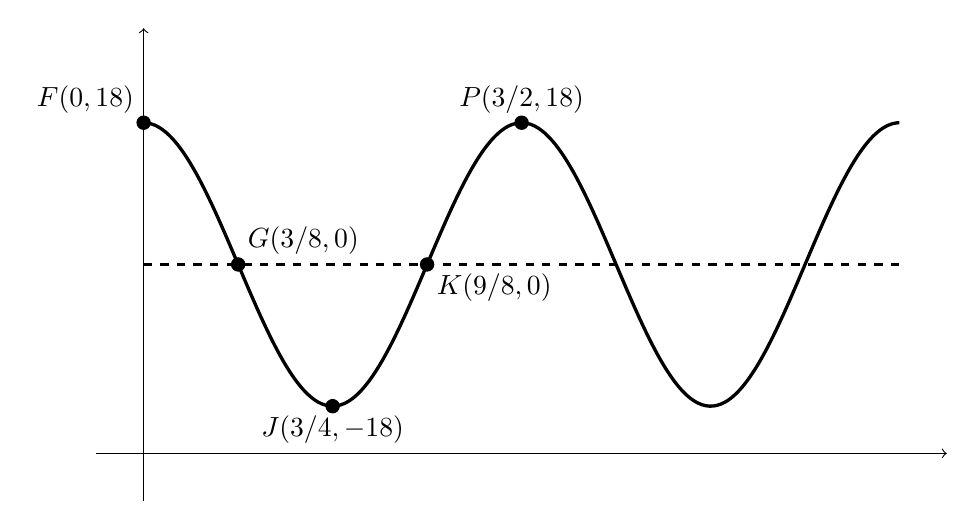
\begin{tikzpicture}[scale=1.2]
    % Draw axes (light)
    \draw[->] (-0.5,0) -- (8.5,0);
    \draw[->] (0,-0.5) -- (0,4.5);
    
    % Draw midline (dashed)
    \draw[dashed, thick] (0,2) -- (8,2);
    
    % Draw sinusoidal curve
    \draw[very thick, domain=0:8, samples=200, smooth] 
        plot (\x, {2 + 1.5*cos(90*\x)});
    
    % Mark and label points with coordinates
    \filldraw (0,3.5) circle (2pt) node[above left] {$F(0, 18)$};
    \filldraw (1,2) circle (2pt) node[above right] {$G(3/8, 0)$};
    \filldraw (2,0.5) circle (2pt) node[below] {$J(3/4, -18)$};
    \filldraw (3,2) circle (2pt) node[below right] {$K(9/8, 0)$};
    \filldraw (4,3.5) circle (2pt) node[above] {$P(3/2, 18)$};
\end{tikzpicture}
\end{center}

\begin{center}
\begin{tabular}{|c|c|}
\hline
$F(0, 18)$ & $P(3/2, 18)$ \\
\hline
$G(3/8, 0)$ & $K(9/8, 0)$ \\
\hline
\multicolumn{2}{|c|}{$J(3/4, -18)$} \\
\hline
\end{tabular}
\end{center}

\subsection*{(B) Constants}

\textbf{Work:}
\begin{itemize}[noitemsep]
    \item Amplitude $a = 18$
    \item Period = $3/2$, so $\displaystyle\frac{2\pi}{b} = \frac{3}{2}$, therefore $\displaystyle b = \frac{4\pi}{3}$
    \item Midline $d = 0$
    \item For cosine starting at maximum: $c = 0$
\end{itemize}

\begin{center}
\begin{tabular}{|l|}
\hline
$a = 18$ \\[10pt]
\hline
$b = 4\pi/3$ \\[10pt]
\hline
$c = 0$ \\[10pt]
\hline
$d = 0$ \\[10pt]
\hline
\end{tabular}
\end{center}

\textbf{Function:} $\displaystyle h(t) = 18 \cos\left(\frac{4\pi}{3} t\right)$

\subsection*{(C) Function Behavior}

\textbf{(i) Answer: c. $h$ is negative and increasing.}

On the interval $J$ to $K$ $(3/4$ to $9/8)$, the function increases from the minimum ($-18$ inches) toward the midline (0 inches). Throughout this interval, $h$ remains negative (to the left of center).

\vspace{0.5cm}
\textbf{(ii) Rate of change description:}

Since $h$ is concave up on the entire interval $(3/4, 9/8)$, the rate of change of $h$ is increasing throughout. The rate starts at zero at the minimum $(t = 3/4)$, becomes increasingly positive, and reaches its maximum value as the pendulum passes through the midline at $t = 9/8$.

\newpage

\section*{Question 4: Trampoline Bounce}

An athlete training for gymnastics is bouncing on a trampoline. At time $t = 0$ seconds, the athlete's feet make contact with the trampoline surface at ground level, modeled by $h(0) = 0$. As the athlete bounces, she reaches a maximum height of 8 feet above the trampoline surface. The athlete completes 48 bounces in 60 seconds. The sinusoidal function $h$ models the height of the athlete's feet above the trampoline surface, in feet, as a function of time $t$ in seconds, $0 \leq t \leq 60$.

\subsection*{(A)}
The graph of $h$ and its dashed midline for two full cycles is shown. Five points, $F$, $G$, $J$, $K$, and $P$, are labeled on the graph. No scale is indicated, and no axes are presented.

Determine possible coordinates $(t, h(t))$ for the five points: $F$, $G$, $J$, $K$, and $P$.

\begin{center}
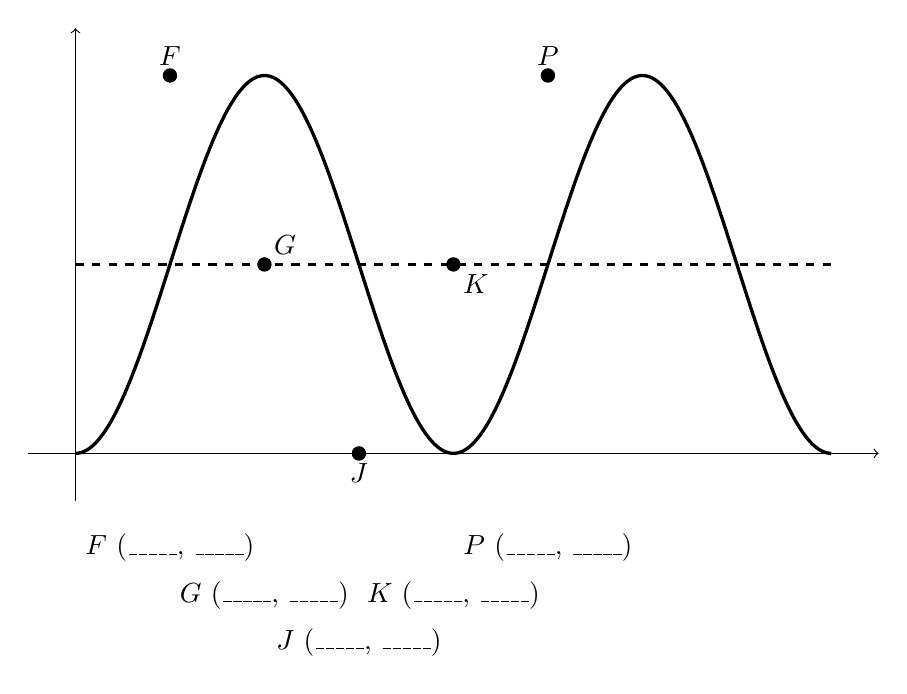
\begin{tikzpicture}[scale=1.2]
    % Draw axes (light)
    \draw[->] (-0.5,0) -- (8.5,0);
    \draw[->] (0,-0.5) -- (0,4.5);
    
    % Draw midline (dashed)
    \draw[dashed, thick] (0,2) -- (8,2);
    
    % Draw sinusoidal curve (starting at minimum)
    \draw[very thick, domain=0:8, samples=200, smooth] 
        plot (\x, {2 - 2*cos(90*\x)});
    
    % Mark and label points (adjusting for minimum at J at origin)
    \filldraw (1,4) circle (2pt) node[above] {$F$};
    \filldraw (2,2) circle (2pt) node[above right] {$G$};
    \filldraw (3,0) circle (2pt) node[below] {$J$};
    \filldraw (4,2) circle (2pt) node[below right] {$K$};
    \filldraw (5,4) circle (2pt) node[above] {$P$};
    
    % Coordinate blanks
    \node at (1,-1) {$F$ (\_\_\_\_\_, \_\_\_\_\_)};
    \node at (5,-1) {$P$ (\_\_\_\_\_, \_\_\_\_\_)};
    \node at (2,-1.5) {$G$ (\_\_\_\_\_, \_\_\_\_\_)};
    \node at (4,-1.5) {$K$ (\_\_\_\_\_, \_\_\_\_\_)};
    \node at (3,-2) {$J$ (\_\_\_\_\_, \_\_\_\_\_)};
\end{tikzpicture}
\end{center}

\subsection*{(B)}
The function $h$ can be written in the form $h(t) = a \sin(b(t + c)) + d$. Find values of constants $a$, $b$, $c$, and $d$.

\begin{center}
\begin{tabular}{|l|}
\hline
$a = $ \underline{\hspace{3cm}} \\[10pt]
\hline
$b = $ \underline{\hspace{3cm}} \\[10pt]
\hline
$c = $ \underline{\hspace{3cm}} \\[10pt]
\hline
$d = $ \underline{\hspace{3cm}} \\[10pt]
\hline
\end{tabular}
\end{center}

\subsection*{(C)}
Refer to the graph of $h$ in part (A). The $t$-coordinate of $F$ is $t_1$, and the $t$-coordinate of $G$ is $t_2$.

\textbf{(i)} On the interval $(t_1, t_2)$, which of the following is true about $h$?

\begin{enumerate}[label=\alph*., leftmargin=1.5cm]
    \item $h$ is positive and increasing.
    \item $h$ is positive and decreasing.
    \item $h$ is negative and increasing.
    \item $h$ is negative and decreasing.
\end{enumerate}

\vspace{0.5cm}
\textbf{(ii)} Describe how the rate of change of $h$ is changing on the interval $(t_1, t_2)$.

\newpage

\section*{Question 4: SOLUTION}

\subsection*{(A) Coordinates}

\textbf{Work:}
\begin{itemize}[noitemsep]
    \item 48 bounces in 60 seconds = 1 bounce every 1.25 seconds
    \item Period = 1.25 seconds = $5/4$ seconds
    \item Max = 8 feet, Min = 0 feet
    \item Amplitude = $(8 - 0)/2 = 4$ feet
    \item Midline = $(8 + 0)/2 = 4$ feet
    \item Increments of $5/16$ seconds between key points
\end{itemize}

\begin{center}
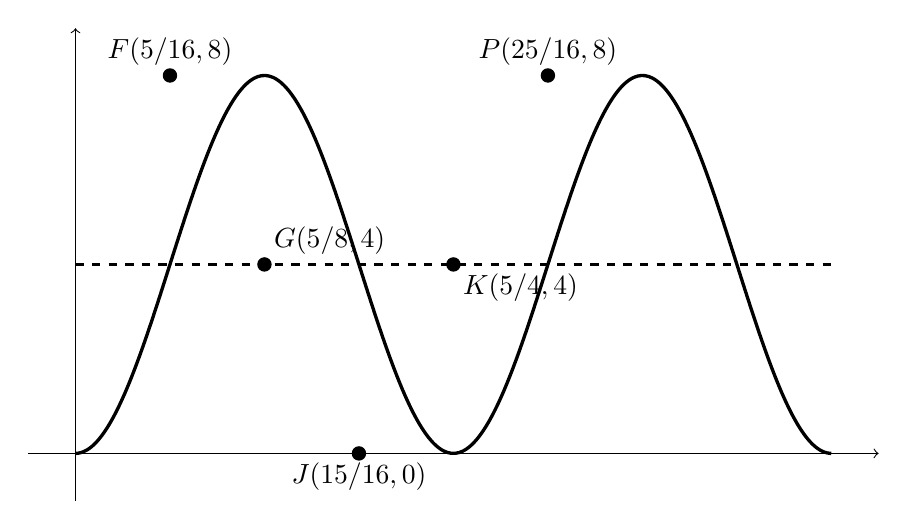
\begin{tikzpicture}[scale=1.2]
    % Draw axes (light)
    \draw[->] (-0.5,0) -- (8.5,0);
    \draw[->] (0,-0.5) -- (0,4.5);
    
    % Draw midline (dashed)
    \draw[dashed, thick] (0,2) -- (8,2);
    
    % Draw sinusoidal curve
    \draw[very thick, domain=0:8, samples=200, smooth] 
        plot (\x, {2 - 2*cos(90*\x)});
    
    % Mark and label points with coordinates
    \filldraw (1,4) circle (2pt) node[above] {$F(5/16, 8)$};
    \filldraw (2,2) circle (2pt) node[above right] {$G(5/8, 4)$};
    \filldraw (3,0) circle (2pt) node[below] {$J(15/16, 0)$};
    \filldraw (4,2) circle (2pt) node[below right] {$K(5/4, 4)$};
    \filldraw (5,4) circle (2pt) node[above] {$P(25/16, 8)$};
\end{tikzpicture}
\end{center}

\begin{center}
\begin{tabular}{|c|c|}
\hline
$F(5/16, 8)$ & $P(25/16, 8)$ \\
\hline
$G(5/8, 4)$ & $K(5/4, 4)$ \\
\hline
\multicolumn{2}{|c|}{$J(15/16, 0)$} \\
\hline
\end{tabular}
\end{center}

\subsection*{(B) Constants}

\textbf{Work:}
\begin{itemize}[noitemsep]
    \item Amplitude $a = 4$
    \item Period = $5/4$, so $\displaystyle\frac{2\pi}{b} = \frac{5}{4}$, therefore $\displaystyle b = \frac{8\pi}{5}$
    \item Midline $d = 4$
    \item For sine with phase shift to start at minimum: $c = -5/16$
\end{itemize}

\begin{center}
\begin{tabular}{|l|}
\hline
$a = 4$ \\[10pt]
\hline
$b = 8\pi/5$ \\[10pt]
\hline
$c = -5/16$ \\[10pt]
\hline
$d = 4$ \\[10pt]
\hline
\end{tabular}
\end{center}

\textbf{Function:} $\displaystyle h(t) = 4 \sin\left(\frac{8\pi}{5}\left(t - \frac{5}{16}\right)\right) + 4$

\textit{OR equivalently:} $\displaystyle h(t) = -4 \cos\left(\frac{8\pi}{5} t\right) + 4$

\subsection*{(C) Function Behavior}

\textbf{(i) Answer: b. $h$ is positive and decreasing.}

On the interval $F$ to $G$ $(5/16$ to $5/8)$, the function decreases from the maximum (8 feet) to the midline (4 feet). Throughout this interval, $h$ remains positive.

\vspace{0.5cm}
\textbf{(ii) Rate of change description:}

Since $h$ is concave down on the entire interval $(5/16, 5/8)$, the rate of change of $h$ is decreasing throughout. The rate starts at zero at the maximum $(t = 5/16)$, becomes increasingly negative, and reaches its most negative value as the athlete approaches the midline at $t = 5/8$.

\newpage

\section*{Question 5: Temperature Variation}

A meteorologist is studying the daily temperature variation in a desert climate. At time $t = 0$ hours (midnight), the temperature is at its minimum of $45^\circ$F, modeled by $T(0) = 45$. As the day progresses, the temperature reaches a maximum of $95^\circ$F in the afternoon. The location experiences one complete temperature cycle every 24 hours. The sinusoidal function $T$ models the temperature, in degrees Fahrenheit, as a function of time $t$ in hours after midnight, $0 \leq t \leq 24$.

\subsection*{(A)}
The graph of $T$ and its dashed midline for two full cycles is shown. Five points, $F$, $G$, $J$, $K$, and $P$, are labeled on the graph. No scale is indicated, and no axes are presented.

Determine possible coordinates $(t, T(t))$ for the five points: $F$, $G$, $J$, $K$, and $P$.

\begin{center}
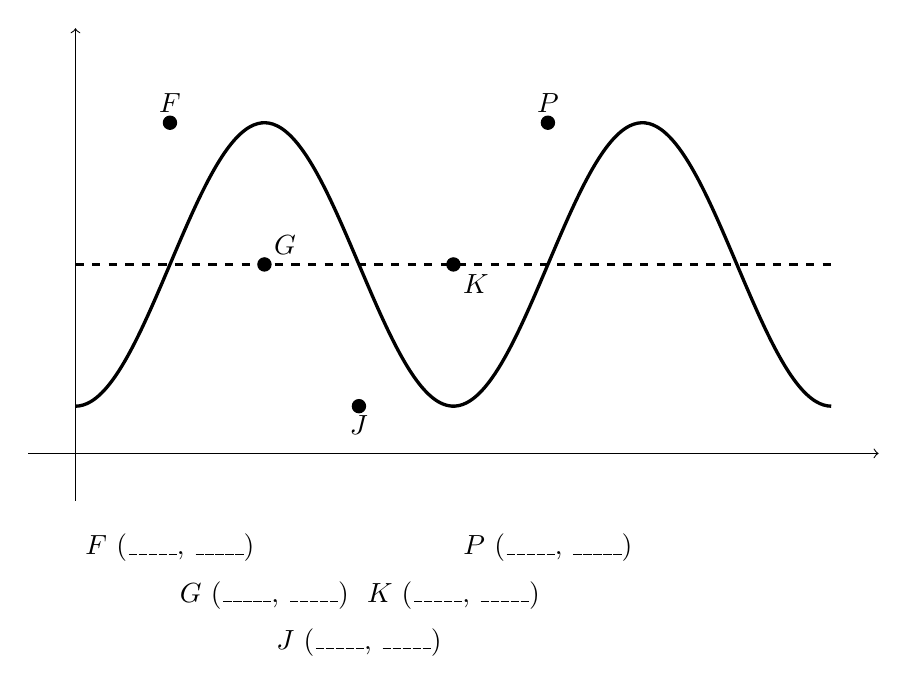
\begin{tikzpicture}[scale=1.2]
    % Draw axes (light)
    \draw[->] (-0.5,0) -- (8.5,0);
    \draw[->] (0,-0.5) -- (0,4.5);
    
    % Draw midline (dashed)
    \draw[dashed, thick] (0,2) -- (8,2);
    
    % Draw sinusoidal curve (starting at minimum)
    \draw[very thick, domain=0:8, samples=200, smooth] 
        plot (\x, {2 - 1.5*cos(90*\x)});
    
    % Mark and label points
    \filldraw (1,3.5) circle (2pt) node[above] {$F$};
    \filldraw (2,2) circle (2pt) node[above right] {$G$};
    \filldraw (3,0.5) circle (2pt) node[below] {$J$};
    \filldraw (4,2) circle (2pt) node[below right] {$K$};
    \filldraw (5,3.5) circle (2pt) node[above] {$P$};
    
    % Coordinate blanks
    \node at (1,-1) {$F$ (\_\_\_\_\_, \_\_\_\_\_)};
    \node at (5,-1) {$P$ (\_\_\_\_\_, \_\_\_\_\_)};
    \node at (2,-1.5) {$G$ (\_\_\_\_\_, \_\_\_\_\_)};
    \node at (4,-1.5) {$K$ (\_\_\_\_\_, \_\_\_\_\_)};
    \node at (3,-2) {$J$ (\_\_\_\_\_, \_\_\_\_\_)};
\end{tikzpicture}
\end{center}

\subsection*{(B)}
The function $T$ can be written in the form $T(t) = a \cos(b(t + c)) + d$. Find values of constants $a$, $b$, $c$, and $d$.

\begin{center}
\begin{tabular}{|l|}
\hline
$a = $ \underline{\hspace{3cm}} \\[10pt]
\hline
$b = $ \underline{\hspace{3cm}} \\[10pt]
\hline
$c = $ \underline{\hspace{3cm}} \\[10pt]
\hline
$d = $ \underline{\hspace{3cm}} \\[10pt]
\hline
\end{tabular}
\end{center}

\subsection*{(C)}
Refer to the graph of $T$ in part (A). The $t$-coordinate of $K$ is $t_1$, and the $t$-coordinate of $P$ is $t_2$.

\textbf{(i)} On the interval $(t_1, t_2)$, which of the following is true about $T$?

\begin{enumerate}[label=\alph*., leftmargin=1.5cm]
    \item $T$ is positive and increasing.
    \item $T$ is positive and decreasing.
    \item $T$ is negative and increasing.
    \item $T$ is negative and decreasing.
\end{enumerate}

\vspace{0.5cm}
\textbf{(ii)} Describe how the rate of change of $T$ is changing on the interval $(t_1, t_2)$.

\newpage

\section*{Question 5: SOLUTION}

\subsection*{(A) Coordinates}

\textbf{Work:}
\begin{itemize}[noitemsep]
    \item 1 cycle in 24 hours
    \item Period = 24 hours
    \item Max = $95^\circ$F, Min = $45^\circ$F
    \item Amplitude = $(95 - 45)/2 = 25^\circ$F
    \item Midline = $(95 + 45)/2 = 70^\circ$F
    \item Increments of $24/4 = 6$ hours between key points
\end{itemize}

\begin{center}
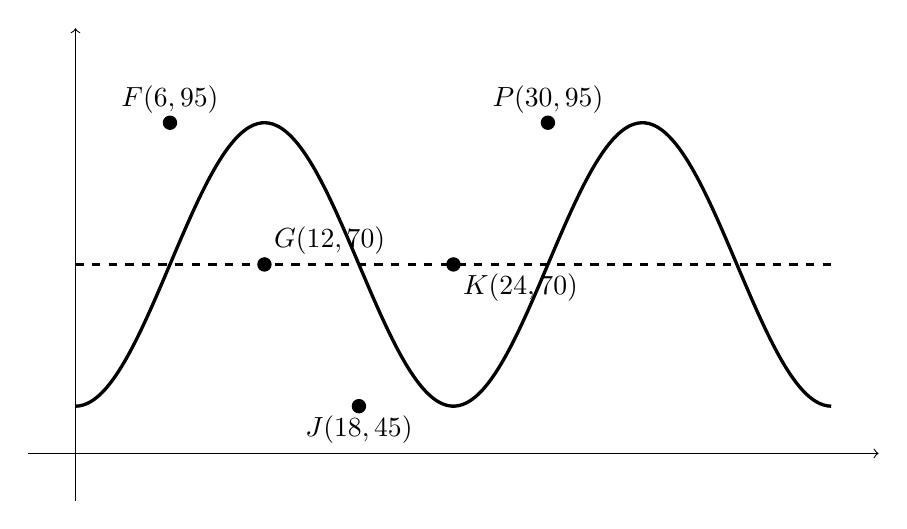
\begin{tikzpicture}[scale=1.2]
    % Draw axes (light)
    \draw[->] (-0.5,0) -- (8.5,0);
    \draw[->] (0,-0.5) -- (0,4.5);
    
    % Draw midline (dashed)
    \draw[dashed, thick] (0,2) -- (8,2);
    
    % Draw sinusoidal curve
    \draw[very thick, domain=0:8, samples=200, smooth] 
        plot (\x, {2 - 1.5*cos(90*\x)});
    
    % Mark and label points with coordinates
    \filldraw (1,3.5) circle (2pt) node[above] {$F(6, 95)$};
    \filldraw (2,2) circle (2pt) node[above right] {$G(12, 70)$};
    \filldraw (3,0.5) circle (2pt) node[below] {$J(18, 45)$};
    \filldraw (4,2) circle (2pt) node[below right] {$K(24, 70)$};
    \filldraw (5,3.5) circle (2pt) node[above] {$P(30, 95)$};
\end{tikzpicture}
\end{center}

\begin{center}
\begin{tabular}{|c|c|}
\hline
$F(6, 95)$ & $P(30, 95)$ \\
\hline
$G(12, 70)$ & $K(24, 70)$ \\
\hline
\multicolumn{2}{|c|}{$J(18, 45)$} \\
\hline
\end{tabular}
\end{center}

\subsection*{(B) Constants}

\textbf{Work:}
\begin{itemize}[noitemsep]
    \item Amplitude: Since we start at minimum, $a = -25$
    \item Period = 24, so $\displaystyle\frac{2\pi}{b} = 24$, therefore $\displaystyle b = \frac{\pi}{12}$
    \item Midline $d = 70$
    \item For cosine starting at minimum: $c = 0$
\end{itemize}

\begin{center}
\begin{tabular}{|l|}
\hline
$a = -25$ \\[10pt]
\hline
$b = \pi/12$ \\[10pt]
\hline
$c = 0$ \\[10pt]
\hline
$d = 70$ \\[10pt]
\hline
\end{tabular}
\end{center}

\textbf{Function:} $\displaystyle T(t) = -25 \cos\left(\frac{\pi}{12} t\right) + 70$

\textit{OR with positive amplitude:} $\displaystyle T(t) = 25 \cos\left(\frac{\pi}{12}(t - 12)\right) + 70$

\subsection*{(C) Function Behavior}

\textbf{(i) Answer: a. $T$ is positive and increasing.}

On the interval $K$ to $P$ (24 to 30), the function increases from the midline $(70^\circ$F) to the maximum $(95^\circ$F). Throughout this interval, $T$ remains positive (all temperatures are above $0^\circ$F).

\vspace{0.5cm}
\textbf{(ii) Rate of change description:}

Since $T$ is concave down on the entire interval $(24, 30)$, the rate of change of $T$ is decreasing throughout. The rate of change starts at its maximum positive value at the midline $(t = 24)$, becomes less positive, and approaches zero as the temperature reaches its maximum at $t = 30$.

\end{document}